% CARGA EL ESTILO CON LAS ESPECIFICACIONES PARA LA TESIS
% SEGUN LA DEP

% La compilacion se debe hacer con la instruccion de Latex a PDF (PDF Texify si se utiliza WinEdt)
% para evitar problemas de tama�o de hoja.
% Todos los archivos de figuras deben estar en formato PDF.
% Al momento de imprimir el documento, se debe hacer sin escala de pagina.

\documentclass[letterpaper,12pt]{cicese}
%%%%%%%%%%%%%%%%%%%%%%%%%%%%%%%%%%%%%%%%%%%%%%%%%%%%%%%%%%%%%%%%%%%%%%%%%%%%%%%%%%%%%%%%%%%%%%%%%%%%%%%%%%%%%%%%%%%%%%%%%%%%%%%%%%%%%%%%%%%%%%%%%%%%%%%%%%%%%%%%%%%%%%%%%%%%%%%%%%%%%%%%%%%%%%%%%%%%%%%%%%%%%%%%%%%%%%%%%%%%%%%%%%%%%%%%%%%%%%%%%%%%%%%%%%%%
\usepackage[letterpaper,left=2.5cm,right=2.5cm,top=3cm,bottom=3cm]{geometry} % ivy
\usepackage{makeidx}
\usepackage{eurosym}
\usepackage{amssymb}
\usepackage{amsmath}
\usepackage{natbib}
\usepackage{cicese}
\usepackage{graphicx}
\usepackage[ansinew]{inputenc}   %este paquete es para poner acentos directamente en el codigo de latex. sin barra
\usepackage{multirow}		% ivy

\setcounter{MaxMatrixCols}{10}
%TCIDATA{OutputFilter=Latex.dll}
%TCIDATA{Version=5.00.0.2552}
%TCIDATA{<META NAME="SaveForMode" CONTENT="2">}
%TCIDATA{LastRevised=Tuesday, June 02, 2009 16:25:45}
%TCIDATA{<META NAME="GraphicsSave" CONTENT="32">}
%TCIDATA{<META NAME="PrintViewPercent" CONTENT="100">}

% Macros for Scientific Word 4.0 documents saved with the LaTeX filter.
% Copyright (C) 2002 Mackichan Software, Inc.

\typeout{TCILATEX Macros for Scientific Word 5.0 <13 Feb 2003>.}
\typeout{NOTICE:  This macro file is NOT proprietary and may be 
freely copied and distributed.}
%
\makeatletter

%%%%%%%%%%%%%%%%%%%%%
% pdfTeX related.
\ifx\pdfoutput\relax\let\pdfoutput=\undefined\fi
\newcount\msipdfoutput
\ifx\pdfoutput\undefined
\else
 \ifcase\pdfoutput
 \else 
    \msipdfoutput=1
    \ifx\paperwidth\undefined
    \else
      \ifdim\paperheight=0pt\relax
      \else
        \pdfpageheight\paperheight
      \fi
      \ifdim\paperwidth=0pt\relax
      \else
        \pdfpagewidth\paperwidth
      \fi
    \fi
  \fi  
\fi

%%%%%%%%%%%%%%%%%%%%%
% FMTeXButton
% This is used for putting TeXButtons in the 
% frontmatter of a document. Add a line like
% \QTagDef{FMTeXButton}{101}{} to the filter 
% section of the cst being used. Also add a
% new section containing:
%     [f_101]
%     ALIAS=FMTexButton
%     TAG_TYPE=FIELD
%     TAG_LEADIN=TeX Button:
%
% It also works to put \defs in the preamble after 
% the \input tcilatex
\def\FMTeXButton#1{#1}
%
%%%%%%%%%%%%%%%%%%%%%%
% macros for time
\newcount\@hour\newcount\@minute\chardef\@x10\chardef\@xv60
\def\tcitime{
\def\@time{%
  \@minute\time\@hour\@minute\divide\@hour\@xv
  \ifnum\@hour<\@x 0\fi\the\@hour:%
  \multiply\@hour\@xv\advance\@minute-\@hour
  \ifnum\@minute<\@x 0\fi\the\@minute
  }}%

%%%%%%%%%%%%%%%%%%%%%%
% macro for hyperref and msihyperref
%\@ifundefined{hyperref}{\def\hyperref#1#2#3#4{#2\ref{#4}#3}}{}

\def\x@hyperref#1#2#3{%
   % Turn off various catcodes before reading parameter 4
   \catcode`\~ = 12
   \catcode`\$ = 12
   \catcode`\_ = 12
   \catcode`\# = 12
   \catcode`\& = 12
   \y@hyperref{#1}{#2}{#3}%
}

\def\y@hyperref#1#2#3#4{%
   #2\ref{#4}#3
   \catcode`\~ = 13
   \catcode`\$ = 3
   \catcode`\_ = 8
   \catcode`\# = 6
   \catcode`\& = 4
}

\@ifundefined{hyperref}{\let\hyperref\x@hyperref}{}
\@ifundefined{msihyperref}{\let\msihyperref\x@hyperref}{}




% macro for external program call
\@ifundefined{qExtProgCall}{\def\qExtProgCall#1#2#3#4#5#6{\relax}}{}
%%%%%%%%%%%%%%%%%%%%%%
%
% macros for graphics
%
\def\FILENAME#1{#1}%
%
\def\QCTOpt[#1]#2{%
  \def\QCTOptB{#1}
  \def\QCTOptA{#2}
}
\def\QCTNOpt#1{%
  \def\QCTOptA{#1}
  \let\QCTOptB\empty
}
\def\Qct{%
  \@ifnextchar[{%
    \QCTOpt}{\QCTNOpt}
}
\def\QCBOpt[#1]#2{%
  \def\QCBOptB{#1}%
  \def\QCBOptA{#2}%
}
\def\QCBNOpt#1{%
  \def\QCBOptA{#1}%
  \let\QCBOptB\empty
}
\def\Qcb{%
  \@ifnextchar[{%
    \QCBOpt}{\QCBNOpt}%
}
\def\PrepCapArgs{%
  \ifx\QCBOptA\empty
    \ifx\QCTOptA\empty
      {}%
    \else
      \ifx\QCTOptB\empty
        {\QCTOptA}%
      \else
        [\QCTOptB]{\QCTOptA}%
      \fi
    \fi
  \else
    \ifx\QCBOptA\empty
      {}%
    \else
      \ifx\QCBOptB\empty
        {\QCBOptA}%
      \else
        [\QCBOptB]{\QCBOptA}%
      \fi
    \fi
  \fi
}
\newcount\GRAPHICSTYPE
%\GRAPHICSTYPE 0 is for TurboTeX
%\GRAPHICSTYPE 1 is for DVIWindo (PostScript)
%%%(removed)%\GRAPHICSTYPE 2 is for psfig (PostScript)
\GRAPHICSTYPE=\z@
\def\GRAPHICSPS#1{%
 \ifcase\GRAPHICSTYPE%\GRAPHICSTYPE=0
   \special{ps: #1}%
 \or%\GRAPHICSTYPE=1
   \special{language "PS", include "#1"}%
%%%\or%\GRAPHICSTYPE=2
%%%  #1%
 \fi
}%
%
\def\GRAPHICSHP#1{\special{include #1}}%
%
% \graffile{ body }                                  %#1
%          { contentswidth (scalar)  }               %#2
%          { contentsheight (scalar) }               %#3
%          { vertical shift when in-line (scalar) }  %#4

\def\graffile#1#2#3#4{%
%%% \ifnum\GRAPHICSTYPE=\tw@
%%%  %Following if using psfig
%%%  \@ifundefined{psfig}{\input psfig.tex}{}%
%%%  \psfig{file=#1, height=#3, width=#2}%
%%% \else
  %Following for all others
  % JCS - added BOXTHEFRAME, see below
    \bgroup
	   \@inlabelfalse
       \leavevmode
       \@ifundefined{bbl@deactivate}{\def~{\string~}}{\activesoff}%
        \raise -#4 \BOXTHEFRAME{%
           \hbox to #2{\raise #3\hbox to #2{\null #1\hfil}}}%
    \egroup
}%
%
% A box for drafts
\def\draftbox#1#2#3#4{%
 \leavevmode\raise -#4 \hbox{%
  \frame{\rlap{\protect\tiny #1}\hbox to #2%
   {\vrule height#3 width\z@ depth\z@\hfil}%
  }%
 }%
}%
%
\newcount\@msidraft
\@msidraft=\z@
\let\nographics=\@msidraft
\newif\ifwasdraft
\wasdraftfalse

%  \GRAPHIC{ body }                                  %#1
%          { draft name }                            %#2
%          { contentswidth (scalar)  }               %#3
%          { contentsheight (scalar) }               %#4
%          { vertical shift when in-line (scalar) }  %#5
\def\GRAPHIC#1#2#3#4#5{%
   \ifnum\@msidraft=\@ne\draftbox{#2}{#3}{#4}{#5}%
   \else\graffile{#1}{#3}{#4}{#5}%
   \fi
}
%
\def\addtoLaTeXparams#1{%
    \edef\LaTeXparams{\LaTeXparams #1}}%
%
% JCS -  added a switch BoxFrame that can 
% be set by including X in the frame params.
% If set a box is drawn around the frame.

\newif\ifBoxFrame \BoxFramefalse
\newif\ifOverFrame \OverFramefalse
\newif\ifUnderFrame \UnderFramefalse

\def\BOXTHEFRAME#1{%
   \hbox{%
      \ifBoxFrame
         \frame{#1}%
      \else
         {#1}%
      \fi
   }%
}


\def\doFRAMEparams#1{\BoxFramefalse\OverFramefalse\UnderFramefalse\readFRAMEparams#1\end}%
\def\readFRAMEparams#1{%
 \ifx#1\end%
  \let\next=\relax
  \else
  \ifx#1i\dispkind=\z@\fi
  \ifx#1d\dispkind=\@ne\fi
  \ifx#1f\dispkind=\tw@\fi
  \ifx#1t\addtoLaTeXparams{t}\fi
  \ifx#1b\addtoLaTeXparams{b}\fi
  \ifx#1p\addtoLaTeXparams{p}\fi
  \ifx#1h\addtoLaTeXparams{h}\fi
  \ifx#1X\BoxFrametrue\fi
  \ifx#1O\OverFrametrue\fi
  \ifx#1U\UnderFrametrue\fi
  \ifx#1w
    \ifnum\@msidraft=1\wasdrafttrue\else\wasdraftfalse\fi
    \@msidraft=\@ne
  \fi
  \let\next=\readFRAMEparams
  \fi
 \next
 }%
%
%Macro for In-line graphics object
%   \IFRAME{ contentswidth (scalar)  }               %#1
%          { contentsheight (scalar) }               %#2
%          { vertical shift when in-line (scalar) }  %#3
%          { draft name }                            %#4
%          { body }                                  %#5
%          { caption}                                %#6


\def\IFRAME#1#2#3#4#5#6{%
      \bgroup
      \let\QCTOptA\empty
      \let\QCTOptB\empty
      \let\QCBOptA\empty
      \let\QCBOptB\empty
      #6%
      \parindent=0pt
      \leftskip=0pt
      \rightskip=0pt
      \setbox0=\hbox{\QCBOptA}%
      \@tempdima=#1\relax
      \ifOverFrame
          % Do this later
          \typeout{This is not implemented yet}%
          \show\HELP
      \else
         \ifdim\wd0>\@tempdima
            \advance\@tempdima by \@tempdima
            \ifdim\wd0 >\@tempdima
               \setbox1 =\vbox{%
                  \unskip\hbox to \@tempdima{\hfill\GRAPHIC{#5}{#4}{#1}{#2}{#3}\hfill}%
                  \unskip\hbox to \@tempdima{\parbox[b]{\@tempdima}{\QCBOptA}}%
               }%
               \wd1=\@tempdima
            \else
               \textwidth=\wd0
               \setbox1 =\vbox{%
                 \noindent\hbox to \wd0{\hfill\GRAPHIC{#5}{#4}{#1}{#2}{#3}\hfill}\\%
                 \noindent\hbox{\QCBOptA}%
               }%
               \wd1=\wd0
            \fi
         \else
            \ifdim\wd0>0pt
              \hsize=\@tempdima
              \setbox1=\vbox{%
                \unskip\GRAPHIC{#5}{#4}{#1}{#2}{0pt}%
                \break
                \unskip\hbox to \@tempdima{\hfill \QCBOptA\hfill}%
              }%
              \wd1=\@tempdima
           \else
              \hsize=\@tempdima
              \setbox1=\vbox{%
                \unskip\GRAPHIC{#5}{#4}{#1}{#2}{0pt}%
              }%
              \wd1=\@tempdima
           \fi
         \fi
         \@tempdimb=\ht1
         %\advance\@tempdimb by \dp1
         \advance\@tempdimb by -#2
         \advance\@tempdimb by #3
         \leavevmode
         \raise -\@tempdimb \hbox{\box1}%
      \fi
      \egroup%
}%
%
%Macro for Display graphics object
%   \DFRAME{ contentswidth (scalar)  }               %#1
%          { contentsheight (scalar) }               %#2
%          { draft label }                           %#3
%          { name }                                  %#4
%          { caption}                                %#5
\def\DFRAME#1#2#3#4#5{%
  \vspace\topsep
  \hfil\break
  \bgroup
     \leftskip\@flushglue
	 \rightskip\@flushglue
	 \parindent\z@
	 \parfillskip\z@skip
     \let\QCTOptA\empty
     \let\QCTOptB\empty
     \let\QCBOptA\empty
     \let\QCBOptB\empty
	 \vbox\bgroup
        \ifOverFrame 
           #5\QCTOptA\par
        \fi
        \GRAPHIC{#4}{#3}{#1}{#2}{\z@}%
        \ifUnderFrame 
           \break#5\QCBOptA
        \fi
	 \egroup
  \egroup
  \vspace\topsep
  \break
}%
%
%Macro for Floating graphic object
%   \FFRAME{ framedata f|i tbph x F|T }              %#1
%          { contentswidth (scalar)  }               %#2
%          { contentsheight (scalar) }               %#3
%          { caption }                               %#4
%          { label }                                 %#5
%          { draft name }                            %#6
%          { body }                                  %#7
\def\FFRAME#1#2#3#4#5#6#7{%
 %If float.sty loaded and float option is 'h', change to 'H'  (gp) 1998/09/05
  \@ifundefined{floatstyle}
    {%floatstyle undefined (and float.sty not present), no change
     \begin{figure}[#1]%
    }
    {%floatstyle DEFINED
	 \ifx#1h%Only the h parameter, change to H
      \begin{figure}[H]%
	 \else
      \begin{figure}[#1]%
	 \fi
	}
  \let\QCTOptA\empty
  \let\QCTOptB\empty
  \let\QCBOptA\empty
  \let\QCBOptB\empty
  \ifOverFrame
    #4
    \ifx\QCTOptA\empty
    \else
      \ifx\QCTOptB\empty
        \caption{\QCTOptA}%
      \else
        \caption[\QCTOptB]{\QCTOptA}%
      \fi
    \fi
    \ifUnderFrame\else
      \label{#5}%
    \fi
  \else
    \UnderFrametrue%
  \fi
  \begin{center}\GRAPHIC{#7}{#6}{#2}{#3}{\z@}\end{center}%
  \ifUnderFrame
    #4
    \ifx\QCBOptA\empty
      \caption{}%
    \else
      \ifx\QCBOptB\empty
        \caption{\QCBOptA}%
      \else
        \caption[\QCBOptB]{\QCBOptA}%
      \fi
    \fi
    \label{#5}%
  \fi
  \end{figure}%
 }%
%
%
%    \FRAME{ framedata f|i tbph x F|T }              %#1
%          { contentswidth (scalar)  }               %#2
%          { contentsheight (scalar) }               %#3
%          { vertical shift when in-line (scalar) }  %#4
%          { caption }                               %#5
%          { label }                                 %#6
%          { name }                                  %#7
%          { body }                                  %#8
%
%    framedata is a string which can contain the following
%    characters: idftbphxFT
%    Their meaning is as follows:
%             i, d or f : in-line, display, or floating
%             t,b,p,h   : LaTeX floating placement options
%             x         : fit contents box to contents
%             F or T    : Figure or Table. 
%                         Later this can expand
%                         to a more general float class.
%
%
\newcount\dispkind%

\def\makeactives{
  \catcode`\"=\active
  \catcode`\;=\active
  \catcode`\:=\active
  \catcode`\'=\active
  \catcode`\~=\active
}
\bgroup
   \makeactives
   \gdef\activesoff{%
      \def"{\string"}%
      \def;{\string;}%
      \def:{\string:}%
      \def'{\string'}%
      \def~{\string~}%
      %\bbl@deactivate{"}%
      %\bbl@deactivate{;}%
      %\bbl@deactivate{:}%
      %\bbl@deactivate{'}%
    }
\egroup

\def\FRAME#1#2#3#4#5#6#7#8{%
 \bgroup
 \ifnum\@msidraft=\@ne
   \wasdrafttrue
 \else
   \wasdraftfalse%
 \fi
 \def\LaTeXparams{}%
 \dispkind=\z@
 \def\LaTeXparams{}%
 \doFRAMEparams{#1}%
 \ifnum\dispkind=\z@\IFRAME{#2}{#3}{#4}{#7}{#8}{#5}\else
  \ifnum\dispkind=\@ne\DFRAME{#2}{#3}{#7}{#8}{#5}\else
   \ifnum\dispkind=\tw@
    \edef\@tempa{\noexpand\FFRAME{\LaTeXparams}}%
    \@tempa{#2}{#3}{#5}{#6}{#7}{#8}%
    \fi
   \fi
  \fi
  \ifwasdraft\@msidraft=1\else\@msidraft=0\fi{}%
  \egroup
 }%
%
% This macro added to let SW gobble a parameter that
% should not be passed on and expanded. 

\def\TEXUX#1{"texux"}

%
% Macros for text attributes:
%
\def\BF#1{{\bf {#1}}}%
\def\NEG#1{\leavevmode\hbox{\rlap{\thinspace/}{$#1$}}}%
%
%%%%%%%%%%%%%%%%%%%%%%%%%%%%%%%%%%%%%%%%%%%%%%%%%%%%%%%%%%%%%%%%%%%%%%%%
%
%
% macros for user - defined functions
\def\limfunc#1{\mathop{\rm #1}}%
\def\func#1{\mathop{\rm #1}\nolimits}%
% macro for unit names
\def\unit#1{\mathord{\thinspace\rm #1}}%

%
% miscellaneous 
\long\def\QQQ#1#2{%
     \long\expandafter\def\csname#1\endcsname{#2}}%
\@ifundefined{QTP}{\def\QTP#1{}}{}
\@ifundefined{QEXCLUDE}{\def\QEXCLUDE#1{}}{}
\@ifundefined{Qlb}{\def\Qlb#1{#1}}{}
\@ifundefined{Qlt}{\def\Qlt#1{#1}}{}
\def\QWE{}%
\long\def\QQA#1#2{}%
\def\QTR#1#2{{\csname#1\endcsname {#2}}}%
\long\def\TeXButton#1#2{#2}%
\long\def\QSubDoc#1#2{#2}%
\def\EXPAND#1[#2]#3{}%
\def\NOEXPAND#1[#2]#3{}%
\def\PROTECTED{}%
\def\LaTeXparent#1{}%
\def\ChildStyles#1{}%
\def\ChildDefaults#1{}%
\def\QTagDef#1#2#3{}%

% Constructs added with Scientific Notebook
\@ifundefined{correctchoice}{\def\correctchoice{\relax}}{}
\@ifundefined{HTML}{\def\HTML#1{\relax}}{}
\@ifundefined{TCIIcon}{\def\TCIIcon#1#2#3#4{\relax}}{}
\if@compatibility
  \typeout{Not defining UNICODE  U or CustomNote commands for LaTeX 2.09.}
\else
  \providecommand{\UNICODE}[2][]{\protect\rule{.1in}{.1in}}
  \providecommand{\U}[1]{\protect\rule{.1in}{.1in}}
  \providecommand{\CustomNote}[3][]{\marginpar{#3}}
\fi

\@ifundefined{lambdabar}{
      \def\lambdabar{\errmessage{You have used the lambdabar symbol. 
                      This is available for typesetting only in RevTeX styles.}}
   }{}

%
% Macros for style editor docs
\@ifundefined{StyleEditBeginDoc}{\def\StyleEditBeginDoc{\relax}}{}
%
% Macros for footnotes
\def\QQfnmark#1{\footnotemark}
\def\QQfntext#1#2{\addtocounter{footnote}{#1}\footnotetext{#2}}
%
% Macros for indexing.
%
\@ifundefined{TCIMAKEINDEX}{}{\makeindex}%
%
% Attempts to avoid problems with other styles
\@ifundefined{abstract}{%
 \def\abstract{%
  \if@twocolumn
   \section*{Abstract (Not appropriate in this style!)}%
   \else \small 
   \begin{center}{\bf Abstract\vspace{-.5em}\vspace{\z@}}\end{center}%
   \quotation 
   \fi
  }%
 }{%
 }%
\@ifundefined{endabstract}{\def\endabstract
  {\if@twocolumn\else\endquotation\fi}}{}%
\@ifundefined{maketitle}{\def\maketitle#1{}}{}%
\@ifundefined{affiliation}{\def\affiliation#1{}}{}%
\@ifundefined{proof}{\def\proof{\noindent{\bfseries Proof. }}}{}%
\@ifundefined{endproof}{\def\endproof{\mbox{\ \rule{.1in}{.1in}}}}{}%
\@ifundefined{newfield}{\def\newfield#1#2{}}{}%
\@ifundefined{chapter}{\def\chapter#1{\par(Chapter head:)#1\par }%
 \newcount\c@chapter}{}%
\@ifundefined{part}{\def\part#1{\par(Part head:)#1\par }}{}%
\@ifundefined{section}{\def\section#1{\par(Section head:)#1\par }}{}%
\@ifundefined{subsection}{\def\subsection#1%
 {\par(Subsection head:)#1\par }}{}%
\@ifundefined{subsubsection}{\def\subsubsection#1%
 {\par(Subsubsection head:)#1\par }}{}%
\@ifundefined{paragraph}{\def\paragraph#1%
 {\par(Subsubsubsection head:)#1\par }}{}%
\@ifundefined{subparagraph}{\def\subparagraph#1%
 {\par(Subsubsubsubsection head:)#1\par }}{}%
%%%%%%%%%%%%%%%%%%%%%%%%%%%%%%%%%%%%%%%%%%%%%%%%%%%%%%%%%%%%%%%%%%%%%%%%
% These symbols are not recognized by LaTeX
\@ifundefined{therefore}{\def\therefore{}}{}%
\@ifundefined{backepsilon}{\def\backepsilon{}}{}%
\@ifundefined{yen}{\def\yen{\hbox{\rm\rlap=Y}}}{}%
\@ifundefined{registered}{%
   \def\registered{\relax\ifmmode{}\r@gistered
                    \else$\m@th\r@gistered$\fi}%
 \def\r@gistered{^{\ooalign
  {\hfil\raise.07ex\hbox{$\scriptstyle\rm\text{R}$}\hfil\crcr
  \mathhexbox20D}}}}{}%
\@ifundefined{Eth}{\def\Eth{}}{}%
\@ifundefined{eth}{\def\eth{}}{}%
\@ifundefined{Thorn}{\def\Thorn{}}{}%
\@ifundefined{thorn}{\def\thorn{}}{}%
% A macro to allow any symbol that requires math to appear in text
\def\TEXTsymbol#1{\mbox{$#1$}}%
\@ifundefined{degree}{\def\degree{{}^{\circ}}}{}%
%
% macros for T3TeX files
\newdimen\theight
\@ifundefined{Column}{\def\Column{%
 \vadjust{\setbox\z@=\hbox{\scriptsize\quad\quad tcol}%
  \theight=\ht\z@\advance\theight by \dp\z@\advance\theight by \lineskip
  \kern -\theight \vbox to \theight{%
   \rightline{\rlap{\box\z@}}%
   \vss
   }%
  }%
 }}{}%
%
\@ifundefined{qed}{\def\qed{%
 \ifhmode\unskip\nobreak\fi\ifmmode\ifinner\else\hskip5\p@\fi\fi
 \hbox{\hskip5\p@\vrule width4\p@ height6\p@ depth1.5\p@\hskip\p@}%
 }}{}%
%
\@ifundefined{cents}{\def\cents{\hbox{\rm\rlap c/}}}{}%
\@ifundefined{tciLaplace}{\def\tciLaplace{\ensuremath{\mathcal{L}}}}{}%
\@ifundefined{tciFourier}{\def\tciFourier{\ensuremath{\mathcal{F}}}}{}%
\@ifundefined{textcurrency}{\def\textcurrency{\hbox{\rm\rlap xo}}}{}%
\@ifundefined{texteuro}{\def\texteuro{\hbox{\rm\rlap C=}}}{}%
\@ifundefined{euro}{\def\euro{\hbox{\rm\rlap C=}}}{}%
\@ifundefined{textfranc}{\def\textfranc{\hbox{\rm\rlap-F}}}{}%
\@ifundefined{textlira}{\def\textlira{\hbox{\rm\rlap L=}}}{}%
\@ifundefined{textpeseta}{\def\textpeseta{\hbox{\rm P\negthinspace s}}}{}%
%
\@ifundefined{miss}{\def\miss{\hbox{\vrule height2\p@ width 2\p@ depth\z@}}}{}%
%
\@ifundefined{vvert}{\def\vvert{\Vert}}{}%  %always translated to \left| or \right|
%
\@ifundefined{tcol}{\def\tcol#1{{\baselineskip=6\p@ \vcenter{#1}} \Column}}{}%
%
\@ifundefined{dB}{\def\dB{\hbox{{}}}}{}%        %dummy entry in column 
\@ifundefined{mB}{\def\mB#1{\hbox{$#1$}}}{}%   %column entry
\@ifundefined{nB}{\def\nB#1{\hbox{#1}}}{}%     %column entry (not math)
%
\@ifundefined{note}{\def\note{$^{\dag}}}{}%
%
\def\newfmtname{LaTeX2e}
% No longer load latexsym.  This is now handled by SWP, which uses amsfonts if necessary
%
\ifx\fmtname\newfmtname
  \DeclareOldFontCommand{\rm}{\normalfont\rmfamily}{\mathrm}
  \DeclareOldFontCommand{\sf}{\normalfont\sffamily}{\mathsf}
  \DeclareOldFontCommand{\tt}{\normalfont\ttfamily}{\mathtt}
  \DeclareOldFontCommand{\bf}{\normalfont\bfseries}{\mathbf}
  \DeclareOldFontCommand{\it}{\normalfont\itshape}{\mathit}
  \DeclareOldFontCommand{\sl}{\normalfont\slshape}{\@nomath\sl}
  \DeclareOldFontCommand{\sc}{\normalfont\scshape}{\@nomath\sc}
\fi

%
% Greek bold macros
% Redefine all of the math symbols 
% which might be bolded	 - there are 
% probably others to add to this list

\def\alpha{{\Greekmath 010B}}%
\def\beta{{\Greekmath 010C}}%
\def\gamma{{\Greekmath 010D}}%
\def\delta{{\Greekmath 010E}}%
\def\epsilon{{\Greekmath 010F}}%
\def\zeta{{\Greekmath 0110}}%
\def\eta{{\Greekmath 0111}}%
\def\theta{{\Greekmath 0112}}%
\def\iota{{\Greekmath 0113}}%
\def\kappa{{\Greekmath 0114}}%
\def\lambda{{\Greekmath 0115}}%
\def\mu{{\Greekmath 0116}}%
\def\nu{{\Greekmath 0117}}%
\def\xi{{\Greekmath 0118}}%
\def\pi{{\Greekmath 0119}}%
\def\rho{{\Greekmath 011A}}%
\def\sigma{{\Greekmath 011B}}%
\def\tau{{\Greekmath 011C}}%
\def\upsilon{{\Greekmath 011D}}%
\def\phi{{\Greekmath 011E}}%
\def\chi{{\Greekmath 011F}}%
\def\psi{{\Greekmath 0120}}%
\def\omega{{\Greekmath 0121}}%
\def\varepsilon{{\Greekmath 0122}}%
\def\vartheta{{\Greekmath 0123}}%
\def\varpi{{\Greekmath 0124}}%
\def\varrho{{\Greekmath 0125}}%
\def\varsigma{{\Greekmath 0126}}%
\def\varphi{{\Greekmath 0127}}%

\def\nabla{{\Greekmath 0272}}
\def\FindBoldGroup{%
   {\setbox0=\hbox{$\mathbf{x\global\edef\theboldgroup{\the\mathgroup}}$}}%
}

\def\Greekmath#1#2#3#4{%
    \if@compatibility
        \ifnum\mathgroup=\symbold
           \mathchoice{\mbox{\boldmath$\displaystyle\mathchar"#1#2#3#4$}}%
                      {\mbox{\boldmath$\textstyle\mathchar"#1#2#3#4$}}%
                      {\mbox{\boldmath$\scriptstyle\mathchar"#1#2#3#4$}}%
                      {\mbox{\boldmath$\scriptscriptstyle\mathchar"#1#2#3#4$}}%
        \else
           \mathchar"#1#2#3#4% 
        \fi 
    \else 
        \FindBoldGroup
        \ifnum\mathgroup=\theboldgroup % For 2e
           \mathchoice{\mbox{\boldmath$\displaystyle\mathchar"#1#2#3#4$}}%
                      {\mbox{\boldmath$\textstyle\mathchar"#1#2#3#4$}}%
                      {\mbox{\boldmath$\scriptstyle\mathchar"#1#2#3#4$}}%
                      {\mbox{\boldmath$\scriptscriptstyle\mathchar"#1#2#3#4$}}%
        \else
           \mathchar"#1#2#3#4% 
        \fi     	    
	  \fi}

\newif\ifGreekBold  \GreekBoldfalse
\let\SAVEPBF=\pbf
\def\pbf{\GreekBoldtrue\SAVEPBF}%
%

\@ifundefined{theorem}{\newtheorem{theorem}{Theorem}}{}
\@ifundefined{lemma}{\newtheorem{lemma}[theorem]{Lemma}}{}
\@ifundefined{corollary}{\newtheorem{corollary}[theorem]{Corollary}}{}
\@ifundefined{conjecture}{\newtheorem{conjecture}[theorem]{Conjecture}}{}
\@ifundefined{proposition}{\newtheorem{proposition}[theorem]{Proposition}}{}
\@ifundefined{axiom}{\newtheorem{axiom}{Axiom}}{}
\@ifundefined{remark}{\newtheorem{remark}{Remark}}{}
\@ifundefined{example}{\newtheorem{example}{Example}}{}
\@ifundefined{exercise}{\newtheorem{exercise}{Exercise}}{}
\@ifundefined{definition}{\newtheorem{definition}{Definition}}{}


\@ifundefined{mathletters}{%
  %\def\theequation{\arabic{equation}}
  \newcounter{equationnumber}  
  \def\mathletters{%
     \addtocounter{equation}{1}
     \edef\@currentlabel{\theequation}%
     \setcounter{equationnumber}{\c@equation}
     \setcounter{equation}{0}%
     \edef\theequation{\@currentlabel\noexpand\alph{equation}}%
  }
  \def\endmathletters{%
     \setcounter{equation}{\value{equationnumber}}%
  }
}{}

%Logos
\@ifundefined{BibTeX}{%
    \def\BibTeX{{\rm B\kern-.05em{\sc i\kern-.025em b}\kern-.08em
                 T\kern-.1667em\lower.7ex\hbox{E}\kern-.125emX}}}{}%
\@ifundefined{AmS}%
    {\def\AmS{{\protect\usefont{OMS}{cmsy}{m}{n}%
                A\kern-.1667em\lower.5ex\hbox{M}\kern-.125emS}}}{}%
\@ifundefined{AmSTeX}{\def\AmSTeX{\protect\AmS-\protect\TeX\@}}{}%
%

% This macro is a fix to eqnarray
\def\@@eqncr{\let\@tempa\relax
    \ifcase\@eqcnt \def\@tempa{& & &}\or \def\@tempa{& &}%
      \else \def\@tempa{&}\fi
     \@tempa
     \if@eqnsw
        \iftag@
           \@taggnum
        \else
           \@eqnnum\stepcounter{equation}%
        \fi
     \fi
     \global\tag@false
     \global\@eqnswtrue
     \global\@eqcnt\z@\cr}


\def\TCItag{\@ifnextchar*{\@TCItagstar}{\@TCItag}}
\def\@TCItag#1{%
    \global\tag@true
    \global\def\@taggnum{(#1)}}
\def\@TCItagstar*#1{%
    \global\tag@true
    \global\def\@taggnum{#1}}
%
%%%%%%%%%%%%%%%%%%%%%%%%%%%%%%%%%%%%%%%%%%%%%%%%%%%%%%%%%%%%%%%%%%%%%
%
\def\QATOP#1#2{{#1 \atop #2}}%
\def\QTATOP#1#2{{\textstyle {#1 \atop #2}}}%
\def\QDATOP#1#2{{\displaystyle {#1 \atop #2}}}%
\def\QABOVE#1#2#3{{#2 \above#1 #3}}%
\def\QTABOVE#1#2#3{{\textstyle {#2 \above#1 #3}}}%
\def\QDABOVE#1#2#3{{\displaystyle {#2 \above#1 #3}}}%
\def\QOVERD#1#2#3#4{{#3 \overwithdelims#1#2 #4}}%
\def\QTOVERD#1#2#3#4{{\textstyle {#3 \overwithdelims#1#2 #4}}}%
\def\QDOVERD#1#2#3#4{{\displaystyle {#3 \overwithdelims#1#2 #4}}}%
\def\QATOPD#1#2#3#4{{#3 \atopwithdelims#1#2 #4}}%
\def\QTATOPD#1#2#3#4{{\textstyle {#3 \atopwithdelims#1#2 #4}}}%
\def\QDATOPD#1#2#3#4{{\displaystyle {#3 \atopwithdelims#1#2 #4}}}%
\def\QABOVED#1#2#3#4#5{{#4 \abovewithdelims#1#2#3 #5}}%
\def\QTABOVED#1#2#3#4#5{{\textstyle 
   {#4 \abovewithdelims#1#2#3 #5}}}%
\def\QDABOVED#1#2#3#4#5{{\displaystyle 
   {#4 \abovewithdelims#1#2#3 #5}}}%
%
% Macros for text size operators:
%
\def\tint{\mathop{\textstyle \int}}%
\def\tiint{\mathop{\textstyle \iint }}%
\def\tiiint{\mathop{\textstyle \iiint }}%
\def\tiiiint{\mathop{\textstyle \iiiint }}%
\def\tidotsint{\mathop{\textstyle \idotsint }}%
\def\toint{\mathop{\textstyle \oint}}%
\def\tsum{\mathop{\textstyle \sum }}%
\def\tprod{\mathop{\textstyle \prod }}%
\def\tbigcap{\mathop{\textstyle \bigcap }}%
\def\tbigwedge{\mathop{\textstyle \bigwedge }}%
\def\tbigoplus{\mathop{\textstyle \bigoplus }}%
\def\tbigodot{\mathop{\textstyle \bigodot }}%
\def\tbigsqcup{\mathop{\textstyle \bigsqcup }}%
\def\tcoprod{\mathop{\textstyle \coprod }}%
\def\tbigcup{\mathop{\textstyle \bigcup }}%
\def\tbigvee{\mathop{\textstyle \bigvee }}%
\def\tbigotimes{\mathop{\textstyle \bigotimes }}%
\def\tbiguplus{\mathop{\textstyle \biguplus }}%
%
%
%Macros for display size operators:
%
\def\dint{\mathop{\displaystyle \int}}%
\def\diint{\mathop{\displaystyle \iint}}%
\def\diiint{\mathop{\displaystyle \iiint}}%
\def\diiiint{\mathop{\displaystyle \iiiint }}%
\def\didotsint{\mathop{\displaystyle \idotsint }}%
\def\doint{\mathop{\displaystyle \oint}}%
\def\dsum{\mathop{\displaystyle \sum }}%
\def\dprod{\mathop{\displaystyle \prod }}%
\def\dbigcap{\mathop{\displaystyle \bigcap }}%
\def\dbigwedge{\mathop{\displaystyle \bigwedge }}%
\def\dbigoplus{\mathop{\displaystyle \bigoplus }}%
\def\dbigodot{\mathop{\displaystyle \bigodot }}%
\def\dbigsqcup{\mathop{\displaystyle \bigsqcup }}%
\def\dcoprod{\mathop{\displaystyle \coprod }}%
\def\dbigcup{\mathop{\displaystyle \bigcup }}%
\def\dbigvee{\mathop{\displaystyle \bigvee }}%
\def\dbigotimes{\mathop{\displaystyle \bigotimes }}%
\def\dbiguplus{\mathop{\displaystyle \biguplus }}%

\if@compatibility\else
  % Always load amsmath in LaTeX2e mode
  \RequirePackage{amsmath}
\fi

\def\ExitTCILatex{\makeatother\endinput}

\bgroup
\ifx\ds@amstex\relax
   \message{amstex already loaded}\aftergroup\ExitTCILatex
\else
   \@ifpackageloaded{amsmath}%
      {\if@compatibility\message{amsmath already loaded}\fi\aftergroup\ExitTCILatex}
      {}
   \@ifpackageloaded{amstex}%
      {\if@compatibility\message{amstex already loaded}\fi\aftergroup\ExitTCILatex}
      {}
   \@ifpackageloaded{amsgen}%
      {\if@compatibility\message{amsgen already loaded}\fi\aftergroup\ExitTCILatex}
      {}
\fi
\egroup

%Exit if any of the AMS macros are already loaded.
%This is always the case for LaTeX2e mode.


%%%%%%%%%%%%%%%%%%%%%%%%%%%%%%%%%%%%%%%%%%%%%%%%%%%%%%%%%%%%%%%%%%%%%%%%%%
% NOTE: The rest of this file is read only if in LaTeX 2.09 compatibility
% mode. This section is used to define AMS-like constructs in the
% event they have not been defined.
%%%%%%%%%%%%%%%%%%%%%%%%%%%%%%%%%%%%%%%%%%%%%%%%%%%%%%%%%%%%%%%%%%%%%%%%%%
\typeout{TCILATEX defining AMS-like constructs in LaTeX 2.09 COMPATIBILITY MODE}
%%%%%%%%%%%%%%%%%%%%%%%%%%%%%%%%%%%%%%%%%%%%%%%%%%%%%%%%%%%%%%%%%%%%%%%%
%  Macros to define some AMS LaTeX constructs when 
%  AMS LaTeX has not been loaded
% 
% These macros are copied from the AMS-TeX package for doing
% multiple integrals.
%
\let\DOTSI\relax
\def\RIfM@{\relax\ifmmode}%
\def\FN@{\futurelet\next}%
\newcount\intno@
\def\iint{\DOTSI\intno@\tw@\FN@\ints@}%
\def\iiint{\DOTSI\intno@\thr@@\FN@\ints@}%
\def\iiiint{\DOTSI\intno@4 \FN@\ints@}%
\def\idotsint{\DOTSI\intno@\z@\FN@\ints@}%
\def\ints@{\findlimits@\ints@@}%
\newif\iflimtoken@
\newif\iflimits@
\def\findlimits@{\limtoken@true\ifx\next\limits\limits@true
 \else\ifx\next\nolimits\limits@false\else
 \limtoken@false\ifx\ilimits@\nolimits\limits@false\else
 \ifinner\limits@false\else\limits@true\fi\fi\fi\fi}%
\def\multint@{\int\ifnum\intno@=\z@\intdots@                          %1
 \else\intkern@\fi                                                    %2
 \ifnum\intno@>\tw@\int\intkern@\fi                                   %3
 \ifnum\intno@>\thr@@\int\intkern@\fi                                 %4
 \int}%                                                               %5
\def\multintlimits@{\intop\ifnum\intno@=\z@\intdots@\else\intkern@\fi
 \ifnum\intno@>\tw@\intop\intkern@\fi
 \ifnum\intno@>\thr@@\intop\intkern@\fi\intop}%
\def\intic@{%
    \mathchoice{\hskip.5em}{\hskip.4em}{\hskip.4em}{\hskip.4em}}%
\def\negintic@{\mathchoice
 {\hskip-.5em}{\hskip-.4em}{\hskip-.4em}{\hskip-.4em}}%
\def\ints@@{\iflimtoken@                                              %1
 \def\ints@@@{\iflimits@\negintic@
   \mathop{\intic@\multintlimits@}\limits                             %2
  \else\multint@\nolimits\fi                                          %3
  \eat@}%                                                             %4
 \else                                                                %5
 \def\ints@@@{\iflimits@\negintic@
  \mathop{\intic@\multintlimits@}\limits\else
  \multint@\nolimits\fi}\fi\ints@@@}%
\def\intkern@{\mathchoice{\!\!\!}{\!\!}{\!\!}{\!\!}}%
\def\plaincdots@{\mathinner{\cdotp\cdotp\cdotp}}%
\def\intdots@{\mathchoice{\plaincdots@}%
 {{\cdotp}\mkern1.5mu{\cdotp}\mkern1.5mu{\cdotp}}%
 {{\cdotp}\mkern1mu{\cdotp}\mkern1mu{\cdotp}}%
 {{\cdotp}\mkern1mu{\cdotp}\mkern1mu{\cdotp}}}%
%
%
%  These macros are for doing the AMS \text{} construct
%
\def\RIfM@{\relax\protect\ifmmode}
\def\text{\RIfM@\expandafter\text@\else\expandafter\mbox\fi}
\let\nfss@text\text
\def\text@#1{\mathchoice
   {\textdef@\displaystyle\f@size{#1}}%
   {\textdef@\textstyle\tf@size{\firstchoice@false #1}}%
   {\textdef@\textstyle\sf@size{\firstchoice@false #1}}%
   {\textdef@\textstyle \ssf@size{\firstchoice@false #1}}%
   \glb@settings}

\def\textdef@#1#2#3{\hbox{{%
                    \everymath{#1}%
                    \let\f@size#2\selectfont
                    #3}}}
\newif\iffirstchoice@
\firstchoice@true
%
%These are the AMS constructs for multiline limits.
%
\def\Let@{\relax\iffalse{\fi\let\\=\cr\iffalse}\fi}%
\def\vspace@{\def\vspace##1{\crcr\noalign{\vskip##1\relax}}}%
\def\multilimits@{\bgroup\vspace@\Let@
 \baselineskip\fontdimen10 \scriptfont\tw@
 \advance\baselineskip\fontdimen12 \scriptfont\tw@
 \lineskip\thr@@\fontdimen8 \scriptfont\thr@@
 \lineskiplimit\lineskip
 \vbox\bgroup\ialign\bgroup\hfil$\m@th\scriptstyle{##}$\hfil\crcr}%
\def\Sb{_\multilimits@}%
\def\endSb{\crcr\egroup\egroup\egroup}%
\def\Sp{^\multilimits@}%
\let\endSp\endSb
%
%
%These are AMS constructs for horizontal arrows
%
\newdimen\ex@
\ex@.2326ex
\def\rightarrowfill@#1{$#1\m@th\mathord-\mkern-6mu\cleaders
 \hbox{$#1\mkern-2mu\mathord-\mkern-2mu$}\hfill
 \mkern-6mu\mathord\rightarrow$}%
\def\leftarrowfill@#1{$#1\m@th\mathord\leftarrow\mkern-6mu\cleaders
 \hbox{$#1\mkern-2mu\mathord-\mkern-2mu$}\hfill\mkern-6mu\mathord-$}%
\def\leftrightarrowfill@#1{$#1\m@th\mathord\leftarrow
\mkern-6mu\cleaders
 \hbox{$#1\mkern-2mu\mathord-\mkern-2mu$}\hfill
 \mkern-6mu\mathord\rightarrow$}%
\def\overrightarrow{\mathpalette\overrightarrow@}%
\def\overrightarrow@#1#2{\vbox{\ialign{##\crcr\rightarrowfill@#1\crcr
 \noalign{\kern-\ex@\nointerlineskip}$\m@th\hfil#1#2\hfil$\crcr}}}%
\let\overarrow\overrightarrow
\def\overleftarrow{\mathpalette\overleftarrow@}%
\def\overleftarrow@#1#2{\vbox{\ialign{##\crcr\leftarrowfill@#1\crcr
 \noalign{\kern-\ex@\nointerlineskip}$\m@th\hfil#1#2\hfil$\crcr}}}%
\def\overleftrightarrow{\mathpalette\overleftrightarrow@}%
\def\overleftrightarrow@#1#2{\vbox{\ialign{##\crcr
   \leftrightarrowfill@#1\crcr
 \noalign{\kern-\ex@\nointerlineskip}$\m@th\hfil#1#2\hfil$\crcr}}}%
\def\underrightarrow{\mathpalette\underrightarrow@}%
\def\underrightarrow@#1#2{\vtop{\ialign{##\crcr$\m@th\hfil#1#2\hfil
  $\crcr\noalign{\nointerlineskip}\rightarrowfill@#1\crcr}}}%
\let\underarrow\underrightarrow
\def\underleftarrow{\mathpalette\underleftarrow@}%
\def\underleftarrow@#1#2{\vtop{\ialign{##\crcr$\m@th\hfil#1#2\hfil
  $\crcr\noalign{\nointerlineskip}\leftarrowfill@#1\crcr}}}%
\def\underleftrightarrow{\mathpalette\underleftrightarrow@}%
\def\underleftrightarrow@#1#2{\vtop{\ialign{##\crcr$\m@th
  \hfil#1#2\hfil$\crcr
 \noalign{\nointerlineskip}\leftrightarrowfill@#1\crcr}}}%
%%%%%%%%%%%%%%%%%%%%%

\def\qopnamewl@#1{\mathop{\operator@font#1}\nlimits@}
\let\nlimits@\displaylimits
\def\setboxz@h{\setbox\z@\hbox}


\def\varlim@#1#2{\mathop{\vtop{\ialign{##\crcr
 \hfil$#1\m@th\operator@font lim$\hfil\crcr
 \noalign{\nointerlineskip}#2#1\crcr
 \noalign{\nointerlineskip\kern-\ex@}\crcr}}}}

 \def\rightarrowfill@#1{\m@th\setboxz@h{$#1-$}\ht\z@\z@
  $#1\copy\z@\mkern-6mu\cleaders
  \hbox{$#1\mkern-2mu\box\z@\mkern-2mu$}\hfill
  \mkern-6mu\mathord\rightarrow$}
\def\leftarrowfill@#1{\m@th\setboxz@h{$#1-$}\ht\z@\z@
  $#1\mathord\leftarrow\mkern-6mu\cleaders
  \hbox{$#1\mkern-2mu\copy\z@\mkern-2mu$}\hfill
  \mkern-6mu\box\z@$}


\def\projlim{\qopnamewl@{proj\,lim}}
\def\injlim{\qopnamewl@{inj\,lim}}
\def\varinjlim{\mathpalette\varlim@\rightarrowfill@}
\def\varprojlim{\mathpalette\varlim@\leftarrowfill@}
\def\varliminf{\mathpalette\varliminf@{}}
\def\varliminf@#1{\mathop{\underline{\vrule\@depth.2\ex@\@width\z@
   \hbox{$#1\m@th\operator@font lim$}}}}
\def\varlimsup{\mathpalette\varlimsup@{}}
\def\varlimsup@#1{\mathop{\overline
  {\hbox{$#1\m@th\operator@font lim$}}}}

%
%Companion to stackrel
\def\stackunder#1#2{\mathrel{\mathop{#2}\limits_{#1}}}%
%
%
% These are AMS environments that will be defined to
% be verbatims if amstex has not actually been 
% loaded
%
%
\begingroup \catcode `|=0 \catcode `[= 1
\catcode`]=2 \catcode `\{=12 \catcode `\}=12
\catcode`\\=12 
|gdef|@alignverbatim#1\end{align}[#1|end[align]]
|gdef|@salignverbatim#1\end{align*}[#1|end[align*]]

|gdef|@alignatverbatim#1\end{alignat}[#1|end[alignat]]
|gdef|@salignatverbatim#1\end{alignat*}[#1|end[alignat*]]

|gdef|@xalignatverbatim#1\end{xalignat}[#1|end[xalignat]]
|gdef|@sxalignatverbatim#1\end{xalignat*}[#1|end[xalignat*]]

|gdef|@gatherverbatim#1\end{gather}[#1|end[gather]]
|gdef|@sgatherverbatim#1\end{gather*}[#1|end[gather*]]

|gdef|@gatherverbatim#1\end{gather}[#1|end[gather]]
|gdef|@sgatherverbatim#1\end{gather*}[#1|end[gather*]]


|gdef|@multilineverbatim#1\end{multiline}[#1|end[multiline]]
|gdef|@smultilineverbatim#1\end{multiline*}[#1|end[multiline*]]

|gdef|@arraxverbatim#1\end{arrax}[#1|end[arrax]]
|gdef|@sarraxverbatim#1\end{arrax*}[#1|end[arrax*]]

|gdef|@tabulaxverbatim#1\end{tabulax}[#1|end[tabulax]]
|gdef|@stabulaxverbatim#1\end{tabulax*}[#1|end[tabulax*]]


|endgroup
  

  
\def\align{\@verbatim \frenchspacing\@vobeyspaces \@alignverbatim
You are using the "align" environment in a style in which it is not defined.}
\let\endalign=\endtrivlist
 
\@namedef{align*}{\@verbatim\@salignverbatim
You are using the "align*" environment in a style in which it is not defined.}
\expandafter\let\csname endalign*\endcsname =\endtrivlist




\def\alignat{\@verbatim \frenchspacing\@vobeyspaces \@alignatverbatim
You are using the "alignat" environment in a style in which it is not defined.}
\let\endalignat=\endtrivlist
 
\@namedef{alignat*}{\@verbatim\@salignatverbatim
You are using the "alignat*" environment in a style in which it is not defined.}
\expandafter\let\csname endalignat*\endcsname =\endtrivlist




\def\xalignat{\@verbatim \frenchspacing\@vobeyspaces \@xalignatverbatim
You are using the "xalignat" environment in a style in which it is not defined.}
\let\endxalignat=\endtrivlist
 
\@namedef{xalignat*}{\@verbatim\@sxalignatverbatim
You are using the "xalignat*" environment in a style in which it is not defined.}
\expandafter\let\csname endxalignat*\endcsname =\endtrivlist




\def\gather{\@verbatim \frenchspacing\@vobeyspaces \@gatherverbatim
You are using the "gather" environment in a style in which it is not defined.}
\let\endgather=\endtrivlist
 
\@namedef{gather*}{\@verbatim\@sgatherverbatim
You are using the "gather*" environment in a style in which it is not defined.}
\expandafter\let\csname endgather*\endcsname =\endtrivlist


\def\multiline{\@verbatim \frenchspacing\@vobeyspaces \@multilineverbatim
You are using the "multiline" environment in a style in which it is not defined.}
\let\endmultiline=\endtrivlist
 
\@namedef{multiline*}{\@verbatim\@smultilineverbatim
You are using the "multiline*" environment in a style in which it is not defined.}
\expandafter\let\csname endmultiline*\endcsname =\endtrivlist


\def\arrax{\@verbatim \frenchspacing\@vobeyspaces \@arraxverbatim
You are using a type of "array" construct that is only allowed in AmS-LaTeX.}
\let\endarrax=\endtrivlist

\def\tabulax{\@verbatim \frenchspacing\@vobeyspaces \@tabulaxverbatim
You are using a type of "tabular" construct that is only allowed in AmS-LaTeX.}
\let\endtabulax=\endtrivlist

 
\@namedef{arrax*}{\@verbatim\@sarraxverbatim
You are using a type of "array*" construct that is only allowed in AmS-LaTeX.}
\expandafter\let\csname endarrax*\endcsname =\endtrivlist

\@namedef{tabulax*}{\@verbatim\@stabulaxverbatim
You are using a type of "tabular*" construct that is only allowed in AmS-LaTeX.}
\expandafter\let\csname endtabulax*\endcsname =\endtrivlist

% macro to simulate ams tag construct


% This macro is a fix to the equation environment
 \def\endequation{%
     \ifmmode\ifinner % FLEQN hack
      \iftag@
        \addtocounter{equation}{-1} % undo the increment made in the begin part
        $\hfil
           \displaywidth\linewidth\@taggnum\egroup \endtrivlist
        \global\tag@false
        \global\@ignoretrue   
      \else
        $\hfil
           \displaywidth\linewidth\@eqnnum\egroup \endtrivlist
        \global\tag@false
        \global\@ignoretrue 
      \fi
     \else   
      \iftag@
        \addtocounter{equation}{-1} % undo the increment made in the begin part
        \eqno \hbox{\@taggnum}
        \global\tag@false%
        $$\global\@ignoretrue
      \else
        \eqno \hbox{\@eqnnum}% $$ BRACE MATCHING HACK
        $$\global\@ignoretrue
      \fi
     \fi\fi
 } 

 \newif\iftag@ \tag@false
 
 \def\TCItag{\@ifnextchar*{\@TCItagstar}{\@TCItag}}
 \def\@TCItag#1{%
     \global\tag@true
     \global\def\@taggnum{(#1)}}
 \def\@TCItagstar*#1{%
     \global\tag@true
     \global\def\@taggnum{#1}}

  \@ifundefined{tag}{
     \def\tag{\@ifnextchar*{\@tagstar}{\@tag}}
     \def\@tag#1{%
         \global\tag@true
         \global\def\@taggnum{(#1)}}
     \def\@tagstar*#1{%
         \global\tag@true
         \global\def\@taggnum{#1}}
  }{}

\def\tfrac#1#2{{\textstyle {#1 \over #2}}}%
\def\dfrac#1#2{{\displaystyle {#1 \over #2}}}%
\def\binom#1#2{{#1 \choose #2}}%
\def\tbinom#1#2{{\textstyle {#1 \choose #2}}}%
\def\dbinom#1#2{{\displaystyle {#1 \choose #2}}}%

% Do not add anything to the end of this file.  
% The last section of the file is loaded only if 
% amstex has not been.
\makeatother
\endinput


\begin{document}

\keywords{Hand gestures recognition, Kinect.}

% Escribe tu nombre, tal y como aparece en los registros
% de Posgrado. De ser necesario, separa con \- las s�labas
% de tu nombre
\autor{Am�rica Ivone Mendoza Morales} %ivy

% Escribe el t�tulo de tu tesis (Si el titulo es mayor de 2 renglones es necesario
% cambiar el valor de espacio vertical para que conserve las dimensiones del margen.
% La modificacion se hace en el archivo cicese.sty en la seccion de la portada que
% ya esta indicado las dimensiones que debe tener para 3 renglones.)
\titulo{Control de computadora basado en gestos en circunstancias de baja iluminaci�n} % ivy

% Para el resumen, escribe aqui el t�tulo en ingl�s
\tituloIN{Light Propagation and Scattering in Confined Systems}

% Aqu� va el nombre de tu programa de posgrado
\posgrado{Ciencias de la Computaci\'on}

% Aqu� va el nombre de orientacion para el que aplique (sino comentarlo)
%\orientacion{con orientaci\'on en \uppercase\expandafter{\'Optica F\'{i}sica}} % ivy

% Escribe aqu� el nombre del posgrado en ingl�s
\posgradoIN{Optics}

% Escribe aqu� el nombre de orientacion para el que aplique (sino comentarlo)
%\orientacionIN{with orientation in \uppercase\expandafter{Physical Optics}}

% El nombre del grado en ingl�s
\gradoIN{Doctor in Sciences}

% Este comando especifica si la tesis es de maestria (usa \mc) o de
% doctorado (usa \dc)
\mc %ivy

% Fecha (mes y a�o) de la defensa de tesis, en espa�ol y en ingles
\fechaexamen{agosto de 2014}\fechaexamenIN{july 2014} % ivy

% Fecha (dia, mes y a�o) de la defensa de tesis para la hoja de firmas
\fechaexamencompleta{28 de agosto de 2014}

% Nombre de tu director de tesis, si tienes codirector repite el comando
\director{Dr. Vitaly Kober} % ivy


% Nombres de los sinodales, en el orden que aparecer�n en la
% p�gina de firmas
\sinodal{Dr.} % ivy

\sinodal{Dr.} %ivy

\sinodal{Dr. } % ivy

% Nombre del Director de Estudios de Posgrado
\dirposgrado{Dr. David Hilario Covarrubias Rosales}
% Nombre del Coordinador del Programa de Posgrado
\cpp{Dr. Ana Isabel Mart\'inez Garc�a} % ivy

% Escribe aqui el nombre del archivo .tex que contiene el texto del
% resumen en espa�ol. Omite escribir la extensi�n .tex
\resumenES{resumen}

% Palabras clave del resumen en espa�ol
\palabrasclave{Reconocimiento de gestos con las manos, Baja iluminaci\'on, Oclusion, Kinect} % ivy

% Escribe aqui el nombre del archivo .tex que contiene el texto del
% resumen en ingl�s. Omite escribir la extensi�n .tex
\resumenIN{Abstract}

% Palabras clave del resumen en ingl�s

% Nombre del archivo .tex con el texto de la dedicatoria, omite
% la extensi�n .tex
\dedicatoria{Dedicatoria}

% Nombre del archivo .tex con el texto de los agradecimientos, omite
% la extensi�n .tex
\agradecimientos{Agradecimientos}

% Este comando crea todas las p�ginas preliminares de la tesis
\preliminares

%----------DOCUMENTO PRINCIPAL-------------------------%

\thispagestyle{empty}
\linespread{1.75}

{	\normalsize
	\chapter{Introducci�n} 

Los humanos para expresarnos utilizamos la escritura y el habla pero generalmente para complementar  usamos como complemento de la expresi�n los gestos corporales de cara, manos, etc. De manera que no es extra\~no que los investigadores de HCI se hayan interesado en los gestos corporales, en especial los gestos realizados con las manos, para crear un ambiente natural entre el usuario y la computadora. 
Pero para realizar esta interacci\'on natural se necesita hacer el reconocimiento de los gestos, esto ha sido cada vez m\'as sencillo gracias al avance de la tecnolog\'ia, en especial con  dispositivos de visi\'on como distintos tipos de c\'amaras, y al crecimiento del procesamiento de las computadoras. Aunque existen diversos m\'etodos para lograr el reconocimiento, no hay alguno que nos pueda dar un reconocimiento totalmente preciso en todas las situaciones que se presentan en el mundo  real.  


La interacci\'on del humano y la computadora (HCI, por sus siglas en \'ingles) es una rama de las ciencias computacionales dedicada al estudio, dise\~no e interacci\'on de un humano con la computadora. El objetivo principal es que, para el humano la interacci\'on entre ellos sea natural.  

Los humanos para expresarnos utilizamos la escritura y el habla pero siempre se utiliza como complemento de la expresi�n los gestos corporales de cara, manos, etc. De manera que no es extra\~no que los investigadores de HCI se hayan interesado en los gestos corporales, en especial los gestos realizados con las manos, para crear un ambiente natural entre el usuario y la computadora. 
Pero para realizar esta interacci\'on natural se necesita hacer el reconocimiento de los gestos, esto ha sido cada vez m\'as sencillo gracias al avance de la tecnolog\'ia, en especial con  dispositivos de visi\'on como distintos tipos de c\'amaras, y al crecimiento del procesamiento de las computadoras. Aunque existen diversos m\'etodos para lograr el reconocimiento, no hay alguno que nos pueda dar un reconocimiento totalmente preciso en todas las situaciones que se presentan en el mundo  real.  

Es por eso que se propone crear un sistema que haga el reconocimiento de gestos con las manos, en situaciones donde existe baja iluminaci\'on y cuando tenemos oclusi\'on causada por los dedos. El sistema se enfoca mayormente  a solucionar los problemas de gestos con las manos que no tienen movimiento, y despu\'es se abordar\'an los gestos con las manos que involucran movimiento. El sistema aplicara los gestos como control de la computadora, esto con ayuda del dispositivo Kinect como  herramienta para capturar la informaci\'on de entrada. 

La propuesta se encuentra dividida por secciones, enseguida se muestra la distibuci\'on de  cada una de estas: la segunda secci\'on se concentra en el marco te\'orico, la tercera muestra la investigaci\'on previa relevante, en la cuarta la importancia de la investigaci\'on, la quinta las limitaciones y suposiciones, la sexta contiene la contribuci\'on al conocimiento, la s\'eptima los objetivos, la octava la metodolog\'ia de la investigaci\'on y por \'ultimo la novena secci\'on  muestra el calendario de actividades que se lleva acabo a lo largo de la investigaci\'on.  
	\chapter{Marco te�rico}

En esta secci�n se encuentran la informaci�n necesaria para entrar en contexto con el tema de reconocimiento de gestos con las manos.  

\section{Reconocimiento de gestos con las manos}

La definici�n de gestos \citep{Mitra2007} son movimientos del cuerpo expresivos y significativos que involucran a los dedos, manos, brazos, cabeza, cara o cuerpo con la intenci�n de transmitir informaci�n relevante o de interactuar con el ambiente. De acuerdo con la literatura \citep{Mitra2007} los gestos con las manos se clasifican en est�ticos y din�micos, los primeros est�n definidos como la posici�n y orientaci�n de la mano en el espacio manteniendo esta pose durante cierto tiempo, por ejemplo para hacer una se\~nal de avent�n, la diferencia de los gestos din�micos es que no se mantiene la pose si no que hay movimiento de la mano, un ejemplo cuando mueves tu mano en se\~nal de adi�s. De aqu� en adelante enti�ndase el t�rmino gestos con las manos, como gestos. 

El reconocimiento de gestos lo podemos dividir en tres fases \cite{Rautaray2012}, detecci�n o segmentaci�n; seguimiento; dependiendo si los gestos son din�micos, por �ltimo la etapa final el reconocimiento del gesto.

Los primeros acercamientos para llevar acabo el reconocimiento de gestos fue usando modelos de contacto \cite{Rautaray2012} y \cite{Nayakwadi2014}, como su nombre lo dice son los que est�n en contacto f�sico con el usuario para capturar la posici�n y el movimiento de la mano, por ejemplo existen los guantes de datos, marcadores de colores, aceler�metros y pantallas multi-touch, aunque estos no son tan aceptados pues entorpecen la naturalidad entre la interacci�n del humano y la computadora.  Posteriormente se desarrollaron los modelos basados en la visi�n, los cuales utilizan c�maras para extraer la informaci�n necesaria para realizar el reconocimiento, desde webcams hasta algunas m�s sofisticadas por ejemplo Kinect. 

A continuaci�n se describen cada uno de estos m�todos,tomando los que est�n basados en la visi�n, ya que estos son mejores para interactuar entre el usuario y la computadora, creando un ambiente natural, pero estos m�todos tienen mayor complejidad para lograr la implementaci�n.

Los m�todos basados en la visi�n se pueden representar por dos modelos \citep{Rautaray2012}, los basados en 3D, da una descripci�n espacial en 3D de la mano, y los basados en apariencia, como su nombre lo dice se basan en la apariencia de la mano. Los modelos basados en apariencia se dividen en dos categor�as, los est�ticos (modelo de silueta, de contorno deformables) y de movimiento (de color y movimiento).

\subsection*{Etapas del reconocimiento de gestos}
Enseguida se describen las etapas del reconocimiento de gestos (detecci�n, seguimiento y reconocimiento), con los m�todos para llevar cada una de estas.  



\subsubsection*{Detecci�n}

En esta etapa se detecta y segmenta la informaci�n relevante de la imagen (la mano), con la del fondo, existen distintos m�todos para obtener dichas caracter�sticas como la de color de la piel, forma, movimiento, entre otras que generalmente son combinaciones de alguna de estas, para obtener un mejor resultado. Enseguida se describe brevemente cada una de estas.  
\begin{itemize}
\item Color de la piel: Se basa principalmente en escoger un espacio del color, es una organizaci�n de colores especifica; como; RGB (rojo, verde, azul), RG (rojo, green), YCrCb (brillo, la diferencia entre el brillo y el rojo, la diferencia entre el brillo y el azul), etc. La desventaja es que si es color de la piel es similar al fondo, la segmentaci�n no es buena, la forma de corregir esta segmentaci�n es suponiendo que el fondo no se mueve con respecto a la c�mara.
\item Forma: Extrae el contorno de las im�genes, si se realiza correctamente se obtiene el contorno de la mano. Aunque si se toman las yemas de los dedos como caracter�sticas, estas pueden ser ocluidas por el resto de la mano, una posible soluci�n es usar m�s de una c�mara.  
\item Valor de pixeles: Usar im�genes en tonos de gris para detectar la mano en base a la apariencia y textura, esto se logra entrenando un clasificador con un conjunto de im�genes.
	\item Modelo 3D: Depende de cual modelo se utilice, son las caracter�sticas de la mano requeridas. 
	\item Movimiento: Generalmente esta se usa con otras formas de detecci�n ya que para utilizarse por s� sola hay que asumir que el �nico objeto con movimiento es la mano.
\end{itemize}

\subsubsection*{Seguimiento}

Consiste en localizar la mano en cada cuadro (imagen). Se lleva acabo usando los m�todos de detecci�n si estos son lo suficientemente r�pidos para detectar la mano cuadro por cuadro. Se explica brevemente los m�todos para llevar a cabo el seguimiento. 
\begin{itemize}
	\item Basado en plantillas: Este se divide en dos categor�as (Caracter�sticas basadas en su correlaci�n y basadas en contorno), que son similares a los m�todos de detecci�n, aunque supone que las im�genes son adquiridas con la frecuencia suficiente para llevar acabo el seguimiento. Caracter�sticas basadas en su correlaci�n, sigue las caracter�sticas a trav�s de cada cuadro, se asume que las caracter�sticas aparecen en mismo vecindario. Basadas en contorno, se basa en contornos deformables, consiste en colocar el contorno cerca de la regi�n de inter�s e ir deformando este hasta encontrar la mano. 
	\item Estimaci�n �ptima: Consiste en usar filtros Kalman, un conjunto de ecuaciones matem�ticas que proporciona una forma  computacionalmente eficiente y recursiva de estimar el estado de un proceso, de una manera que minimiza la media de un error cuadr�tico, el filtro soporta estimaciones del pasado, presente y futuros estados, y puede hacerlo incluso cuando la naturaleza precisa del modelo del sistema es desconocida;  para hacer la detecci�n de caracter�sticas en la trayectoria. 
	\item Filtrado de part�culas: Un m�todo de estimaci�n del estado de un sistema que cambia a lo largo del tiempo, este se compone de un conjunto de part�culas (muestras) con pesos asignados, las part�culas son estados posibles del proceso. Es utilizado cuando no se distingue bien la mano en la imagen. Por medio de part�culas localiza la mano la desventaja es que se requieren demasiadas part�culas, y el seguimiento se vuelve imposible. 
	\item Camshift: Busca el objetivo, en este caso la mano, encuentra el patr�n de distribuci�n mas similar en una secuencia de im�genes, la distribuci�n puede basada en el color. 
\end{itemize}

\subsubsection*{Reconocimiento}

Es la clasificaci�n del gesto, la etapa final del reconocimiento, la clasificaci�n se puede hacer dependiendo del gesto. Para gestos est�ticos basta con usar alg�n clasificador o empatar el gesto con una plantilla. En los din�micos se requiere otro tipo de algoritmos de aprendizaje de m�quina. A continuaci�n se encuentran los principales m�todos para llevar acabo el reconocimiento del gestos. 
\begin{itemize}
	\item K-medias: Consiste en determinar los $k$ puntos llamados centros para minimizar el error de agrupamiento, que es la suma de las distancias de todo los puntos al centro de cada grupo. El algoritmo empieza localizando aleatoriamente $k$ grupos en el espacio espectral. Cada p\'ixel en la imagen de entrada es entonces asignadas al centro del grupo mas cercano  
	\item {K-vecinos cercanos} (KNN, por sus siglas en ingl\'es): 
	Este es un m�todo para clasificar objetos basado en las muestras de entrenamiento en el espacio de caracter�sticas. 
	\item Desplazamiento de medias: Es un m�todo iterativo que encuentra el m�ximo en una funci�n de densidad dada una muestra estad�stica de los datos.
	\item M�quinas de soporte vectorial (SVM, por sus siglas en ingl\'es). Consiste en un mapeo no lineal de los datos de entrada a un espacio de dimensi\'on m\'as grande, donde los datos pueden ser separados de forma lineal.  
	\item Modelo oculto de Markov (HMM, por sus siglas en ingl\'es) es definido como un conjunto de estados donde un estado es el estado inicial, un conjunto de s�mbolos de salida y un conjunto de estados de transici�n. En el reconocimiento de gestos se puede caracterizar a    los estados como un conjunto de las posiciones de la mano; las  transiciones de los estados como la probabilidad de transici�n de cierta posici�n de la mano a otra; el s�mbolo de salida como una postura especifica y la secuencia de los s�mbolos de salida como  el gesto de la mano.   
	\item Redes neuronales con retraso: Son una clase de redes neuronales artificiales que se enfocan en datos continuos, haciendo que el sistema sea adaptable para redes en linea y les da ventajas sobre aplicaciones en tiempo real. 
\end{itemize} 


\section{M�tricas de distancia}

Existen diversas m�tricas, formas de medici�n, de distancia que nos sirven para comparar im�genes como: la distancia Euclidiana, Mahalanobis, Manhattan y Hausdorff. A conti\-nuaci�n se mencionan las dos primeras ya que son  utilizadas con mayor frecuencia. 

\subsection*{Distancia Euclidiana} 
Sea $X$, $Y$ dos im�genes, la distancia euclidiana se define como:

$$d(X,Y)=\sqrt{(X-Y)^t(X-Y)}$$.

\subsection*{Distancia Mahalanobis}


$$d(X,Y)=\sqrt{(X- Y)^t \Sigma^{-1}(X - Y)$$,

donde $\Sigma^{-1}=\sum_{k=1}^{N}\frac{(x_k-x_m)(y_k-y_m)}{N}$, $x_m$, $y_m$ es la media.  
\section{Fusi�n de datos}

La fusi�n de datos de multi-sensores se define \citep{Mitchell2012} la teor�a, t�cnicas y herramientas que son usadas para combinar datos del sensor, o datos provenientes de las lecturas del sensor, a una formato com�n. 
Se puede clasificar la fusi�n de multi-sensores de diferentes maneras como:  aspecto del sistema se fusiona,  debido a la configuraci�n del sensor y a las caracter�sticas de entrada y salida. 
Enseguida se describe brevemente la  clasificaci�n dependiendo de que aspecto del sistema se fusiona. 

\subsection*{Fusi�n a trav�s del sensor} Se realiza con cierto n\'umero de sensores que miden la misma propiedad.
\subsection*{Fusi�n a trav�s de atributos} Se lleva acabo con cierto n\'umero de sensores que miden diferentes cantidades asociadas a mismo experimento. 
\subsection*{Fusi�n a trav�s del dominio} Cierto n\'umero de sensores miden el mismo atributo sobre en diferentes rangos o dominios. 
\subsection*{Fusi�n a trav�s del tiempo} En este tipo de fusi�n las medidas recientes son fusionadas con informaci�n obtenida ante\-riormente.
\end{itemize}





	\chapter{Investigaci\'on previa relevante}

La secci�n anterior explica los distintos enfoques para llevar acabo el reconocimiento de gestos, a continuaci�n se encuentran los trabajos relevantes de cada uno de estos enfoques. 

\section{Modelos de contacto}

\citep{Yoon2012} propone un modelo de mezclas adaptativo, usando un guante de datos, la principal limitante para este sistema es que solo reconoce gestos est�ticos. 

Aunque estos sistemas nos evitan algunos problemas que son consecuencia de los modelos basados en la visi�n, nos son perfectos, lo cual veremos enseguida.  

Uno de los dispositivos recientes es MYO \footnote{https://www.thalmic.com/en/myo/}, aunque de este se hablar\'a en la ultima parte de esta secci\'on. 

Como se describi\'o en la secci\'on anterior en los modelos de contacto la principal limitante es el uso de dispositivos en el cuerpo para el reconocimiento de los gestos, por esta raz\'on la mayor\'ia de los sistemas para el reconocimiento estan enfocados en modelos basados en visi\'on. Por lo que resulta natural que la investigaci\'on propuesta tome un enfoque basado en la visi\'on.

\section{Modelos basados en la visi\'on}  

\cite{Premaratne2013} realizan un modelo de reconocimiento de gestos est\'atico y din\'amico basados en el algoritmo de Lucas-Kanade. Las principales ventajas de este m\'etodo son que es invariante a rotaci\'on, escala y al fondo. Aunque el modelo es afectado por los cambios en la iluminaci\'on.

\citep{Huang2011}, propone un m�todo para calculas gestos est�ticos y din�micos usando los filtros Gabor y haciendo una estimaci�n del \'angulo en el que se encuentra la mano. Las principales ventajas son que el sistema funciona con cambios en la iluminaci\'on y es robusto a la rotaci\'on y escala. La desventaja es que el problema de oclusi\'on no es tratado.

\citep{MohdAsaari2014} hacen el seguimiento de la mano para identificar los gestos din\'amicos usando los filtros adaptativos Kalman y el m\'etodo Eigenhand. Con esta combinaci\'on obtienen un excelente resultado pues el sistema es robusto a la iluminaci\'on, cambio de pose, y a la oclusi\'on causada la mano oculta por alg\'un objeto en movimiento. 

 

A pesar que la mayor�a de los modelos vistos en la parte de arriba solucionan muchos de los problemas de los modelos basados en la visi\'on. Ninguno de ellos puede resolver el problema de iluminaci\'on y oclusi\'on, formada por lo dedos. All\'i la importancia de la investigaci\'on propuesta, pues dar\'a soluci\'on a estos inconvenientes al momento de reconocer los gestos.
 
\section{Sistemas comerciales}

Existen dispositivos como: Leap Motion \footnote{https://www.leapmotion.com/}, MYO, y software, como Flutter \footnote{https://flutterapp.com/}, que realizan el reconocimiento de gestos, y estos los utilizan como reemplazo del rat\'on de la computadora. 
 
Leap Motion es un dispositivo que detecta los movimientos de manos y dedos por medio de sensores infrarrojos. Leap Motion es robusto con el fondo, escala y rotaci\'on,  pero no cuando existe oclusi\'on pues cuando se realiza un zoom, como el que se hace en cualquier dispositivo touch, produce un error, y se presenta cuando un dedo es cubierto por otro, un problema grave es que tiene problemas de reconocimiento en circunstancias normales de luz.  

MYO este dispositivo, solo se encuentra en pre-ordenamiento, detecta los impulsos el\'ectricos de tus m\'usculos mediante tres sensores, giroscopio, aceler\'ometro y magnet\'ometros. MYO es un brazalete  que promete controlar la computadora y dispositivos tales como el celular o la tableta. La principal desventaja del sensor es que gestos involuntarios pueden producir acciones no deseadas.

Flutter  es un software que reconoce cuatro gestos est\'aticos detectando la palma de la mano, usando la c\'amara web como dispositivo de entrada. Flutter permite controlar aplicaciones multimedia de la computadora. 	Las limitaciones del software son que solo reconoce gestos est\'aticos, realiza acciones no deseadas al hacer gestos involuntarios y no siempre reconoce los gestos. 

Aunque estos dispositivos y software para reconocer gestos  solucionan algunos problemas importantes en el \'area, sigue existiendo el problema de oclusi\'on  e iluminaci\'on. De all� la importancia que existan modelos que puedan resolver estos problemas se presentan frecuentemente en el reconocimiento. 
	\chapter{Importancia de la investigaci\'on}

La mayor�a de los sistemas que hacen reconocimiento de gestos con las manos no hacen uso de informaci�n 3D, mientras que los que si lo hacen no toman en cuenta el gran potencial que se encuentra en la mezcla de informaci�n 3D de varios puntos de visi�n. De manera que la importancia de este trabajo consiste en explorar nuevas m�todos basados en la utilizaci�n de informaci�n 3D obtenida de dos sensores de profundidad que recuperan informaci�n de una misma escena.

La HCI, se dedica a que la interacci\'on entre el usuario y la computadora sea de forma natural  y amigable. Y una manera de lograr u obtener un acercamiento a esta interacci\'on es con el reconocimiento de gestos,  en especial el de las manos. Aunque existen diversos m\'etodos para realizar el reconocimiento, estos funcionan en distintas circunstancias como los son el fondo est\'atico, fondo complejo, baja iluminaci\'on, oclusi\'on del gesto. \citep{Sgouropoulos2013}, \citep{Murthy2009}

Realidad aumentada, el mouse y el teclado no siempre pueden transmitir la informaci\'on necesaria cuando se trata de obtener un modelo 3D en la computadora por eso es necesario encontrar una manera de transmitir esta informaci\'on y que mejor que con el uso de un espacio 3D por lo que en este caso es de gran utilidad el reconocimiento de gestos con las manos. \citep{Reifinger2007} 

	\chapter{Limitaciones y suposiciones}
 
Gran porcentaje de los trabajos realizados anteriormente para el reconocimiento de gestos basado en el modelo de la visi\'on  utilizan c\'amaras digitales o c\'amaras web, en la investigaci\'on se utilizar\'a el dispositivo Kinect, para tomar la informaci\'on de entrada (RGB, infrarroja y profundidad). De tal manera que las limitaciones del sistema propuesto est\'an dadas por las caracter�sticas dicho dispositivo, tales como la distancia a la que se encontrara, la resoluci\'on de las im\'agenes, en especial a la baja resoluci\'on de la informaci\'on infrarroja. 
Tambi\'en el sistema depende de dos Kinect, que se utilizar\'an en el caso que exista oclusi\'on. \\
Otra limitante es el n�mero de gestos que podra reconocer el sistema.

Se supone el �rea de trabajo como un cuarto est�ndar con buena iluminaci�n (enfocado a pruebas con la c�mara RGB del sistema Kinect)


	\chapter{Contribuci\'on  al conocimiento}

El sistema a desarrollar debe ser capaz de reconocer diversos gestos con la mano, tanto est�ticos como din�micos, haciendo uso de la informaci�n 3D generada por dos sensores de profundidad, mezclando dicha informaci�n
se pretende dar soluci�n a los problemas de baja iluminaci�n y oclusi�n, que se presentan al hacer el reconocimiento de gestos.
Lo anterior pretende hacer conciencia del potencial de el uso de la informaci�n tridimensional en sistemas similares apoyados en dispositivos de recopilaci�n de datos 3D en tiempo real. 

La aportaci\'on en las \'areas de HCI y realidad aumentada ya que con el modelo propuesto se podr\'a dar soluci\'on a algunas de las limitaciones importantes para el reconocimiento de gestos. 

	\chapter{Objetivos}

\section{Objetivo general}

Desarrollar un sistema que permita controlar la computadora haciendo uso de gestos con las manos, est�ticos y din�micos. El sistema debe ser robusto, funcionar en circunstancias de baja iluminaci�n, cuando exista oclusi�n en gestos din�micos.

\section{Objetivos espec\'ificos}

\begin{enumerate}
	\item Identificar los m\'etodos actuales de reconocimiento de gestos, est\'aticos y din\'amicos cuando existe baja iluminaci�n  y en el caso de los gestos din�micos cuando existe oclusi�n. 
	\item  Obtener conocimiento acerca del funcionamiento de sistema Microsoft Kinect.
	\item Desarrollar un sistema de reconocimiento de gestos est�ticos y din�micos, fusionando la informaci�n de los sensores de  profundidad del dispositivo kinect. El sistema desarrollado deber� funcionar en circunstancias de baja iluminaci�n y tambi�n cuando existe oclusi�n, causada por los dedos. 
	\item Analizar el sistema dise\~nado, en cuanto a su eficiencia presentada en base al reconocimiento de los gestos y tiempo de respuesta, en circunstancias de baja iluminaci�n y oclusi�n. En el an�lisis del sistema se usara informaci�n real.  
	\item Comparar los modelos propuestos  con los existentes, en base al tiempo de respuesta y la eficiencia en cuanto al reconocimiento del gesto. 
\end{enumerate} 


\section{Preguntas de investigaci\'on}

\begin{enumerate}
	\item >Cu�l es el desempe�o de las t�cnicas desarrolladas al compararlas con las t�cnicas cl�sicas?
	\item >Es posible mejorar el desempe�o de las t�cnicas cl�sicas usando informaci�n de mapas de profundidad multi-vista?
	\item >Es posible garantizar un grado de confiabilidad de los resultados?
\end{enumerate}
	\chapter{Metodolog\'ia de la investigaci\'on}

\begin{enumerate}
	\item Realizar una revisi\'on bibliogr\'afica de los m\'etodos existentes de reconocimiento de gestos e identificar los principales m�todos con base en los problemas que atacan. 
	\item Conocer el funcionamiento del dispositivo Microsoft Kinect  y realizar algunas pruebas con los sensores y el programa.
	\item Estudiar  y comprender los modelos basados en visi\'on usados para el reconocimiento de gestos, los cuales fusionan diferentes tipos de informaci\'on de entrada. 
	\item Crear una base de datos con los gestos necesarios para el sistema. 
	\item Implementar los modelos relevantes de fusi�n, estudiados previamente.  
	\item Generaci�n de un mapa de profundidad de dos mapas de profundidad, el mapa generado deber� contar con mayor informaci�n - raz�n de se�al a ruido (SNR) de la escena.
	\item Desarrollar un sistema de reconocimiento de gestos est�ticos y din�mico utilizando informaci�n de los sensores de profundidad.
	\item Probar y evaluar  los modelos desarrollados en circunstancias distintas de iluminaci�n en base al tiempo de respuesta, a la precisi\'on del reconocimiento del gesto. La informaci�n para la evaluaci�n del sistema ser�n muestras reales.   
	\item Analizar y evaluar los modelos existentes conforme al tiempo de respuesta y la precisi\'on del reconocimiento del gesto.
\end{enumerate}





	\chapter{Calendario de actividades}

\begin{figure}[h]
	\centering
		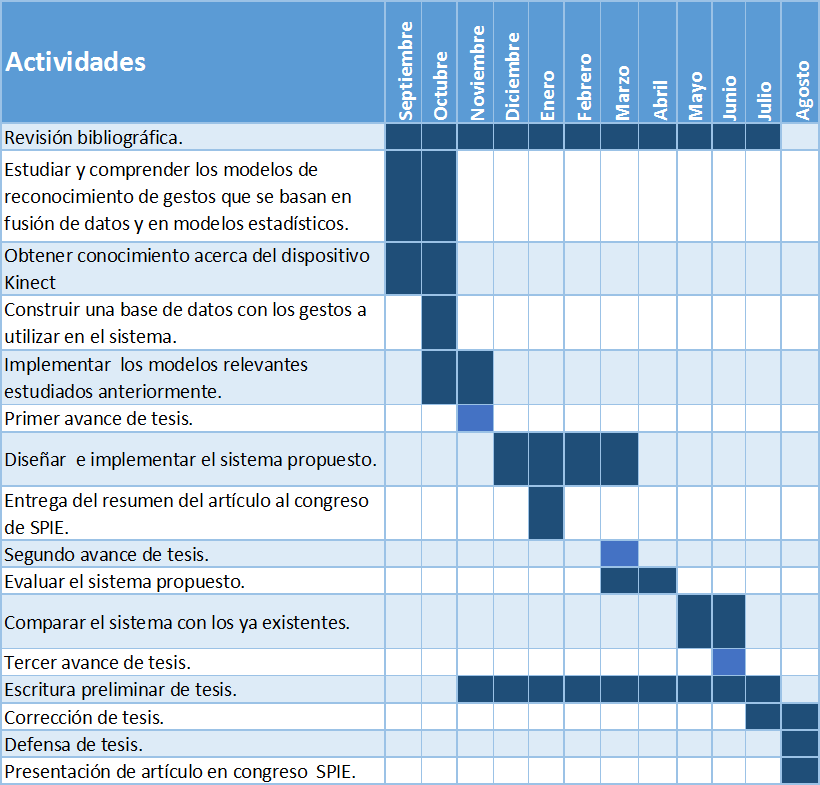
\includegraphics[height=160mm]{Figures/cal.png}
	\caption{Calendario de actividades del proyecto de investigaci�n}
\end{figure}

	\newpage }

\linespread{1.0}

\addcontentsline{toc}{chapter}{\normalsize\expandafter{Referencias}}
{\normalsize
 \bibliographystyle{cicese}
 \bibliography{referencias} }

%\linespread{1.75}
%{\normalsize
%TCIMACRO{\QSubDoc{Include Apendice}{\appendix{}

\chapter{Apéndice} \label{chap:apendA}
%
\setcounter{figure}{0}
\numberwithin{figure}{chapter}
\numberwithin{table}{section}

El apéndice...} }%
%BeginExpansion
%\chapter{Calendario de actividades}

\begin{figure}[h]
	\centering
		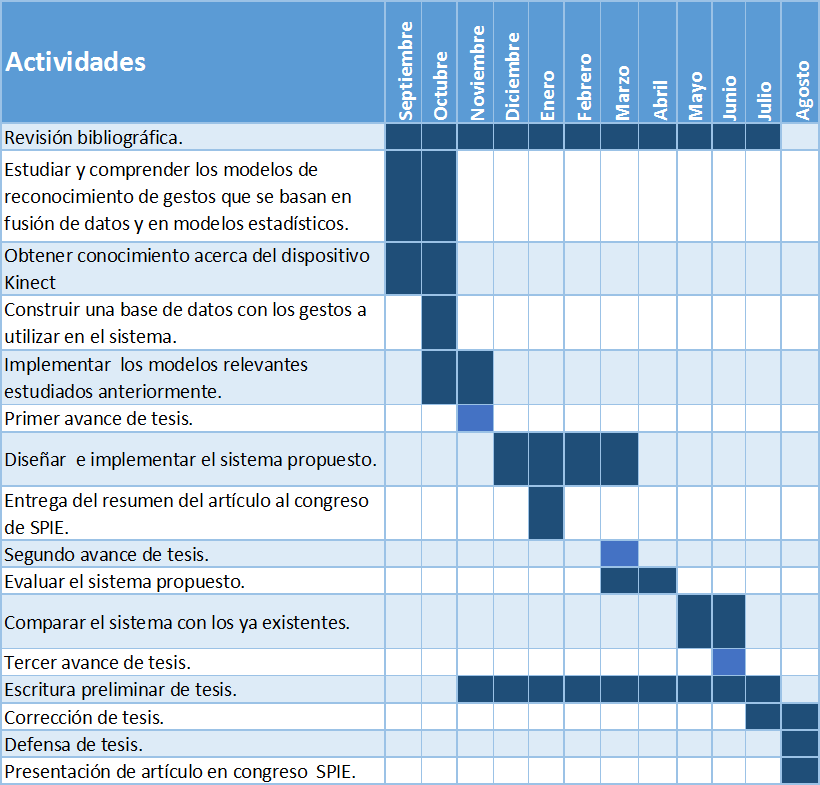
\includegraphics[height=160mm]{Figures/cal.png}
	\caption{Calendario de actividades del proyecto de investigaci�n}
\end{figure}

%EndExpansion
%\newpage }


\end{document}